In descriptive statistics, given a set of random points
$\{x_i\}_{i=1}^{N} \subset \mathbb{R}^n$, the sample mean
$\bar x = \frac{1}{N}\sum_{i=1}^{N} x_i$ is used to estimate the central
tendency of the data. The mean is the quantity that minimizes the sum of square distances.

In the functional case, the mean function will have this property thus if
$\{f_i\}_{i=1}^{N} \subset \mathbb{L}^2$ is a set of functional observations,
their mean $\bar f(t) = \frac{1}{N}\sum_{i=1}^{N} f_i(t)$ will minimize
$\sum_{i=1}^{N}\|f_i - \bar f\|_{\mathbb{L}^2}^2$.

We are interested in extend this idea to general metrics spaces.
Let $(X, d)$ be a metric space and $\{x_i\}_{i=1}^{N}$ random points in $X$.
The Fréchet variance of a point $p \in X$ as $\Psi(p)=\sum_{i=1}^{N} d^{2}\left(p, x_{i}\right)$.

\begin{figure}[Karcher mean of dataset]{FIG:KARCHER}{Karcher mean of dataset}
	\subfigure[SBFIG:KARCHER1]{Dataset of unimodal samples}{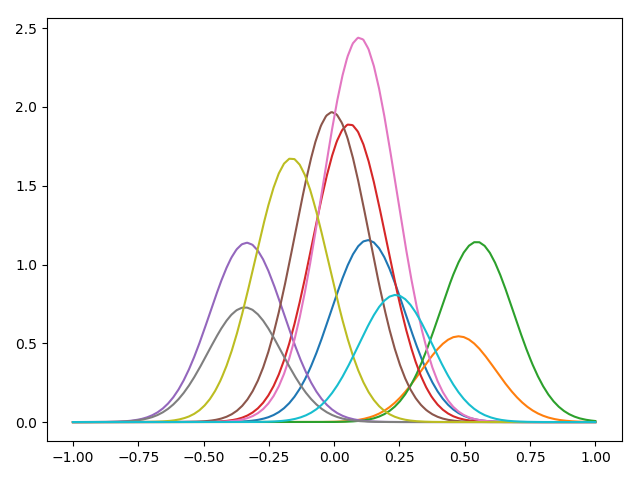
\includegraphics[width=7cm]{unimodal-dataset}} \quad
	\subfigure[SBFIG:KARCHER2]{Usual mean and Karcher mean on $\mathscr{A}$}{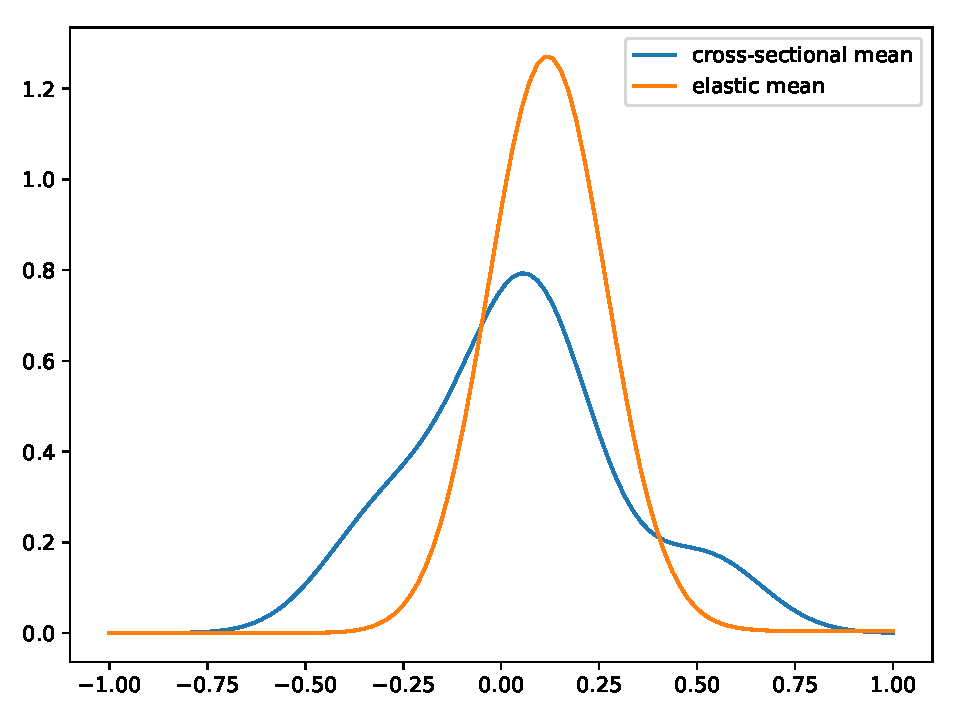
\includegraphics[width=7cm]{means}} \\
	\subfigure[SBFIG:RANK1]{Ranked by elastic distance}{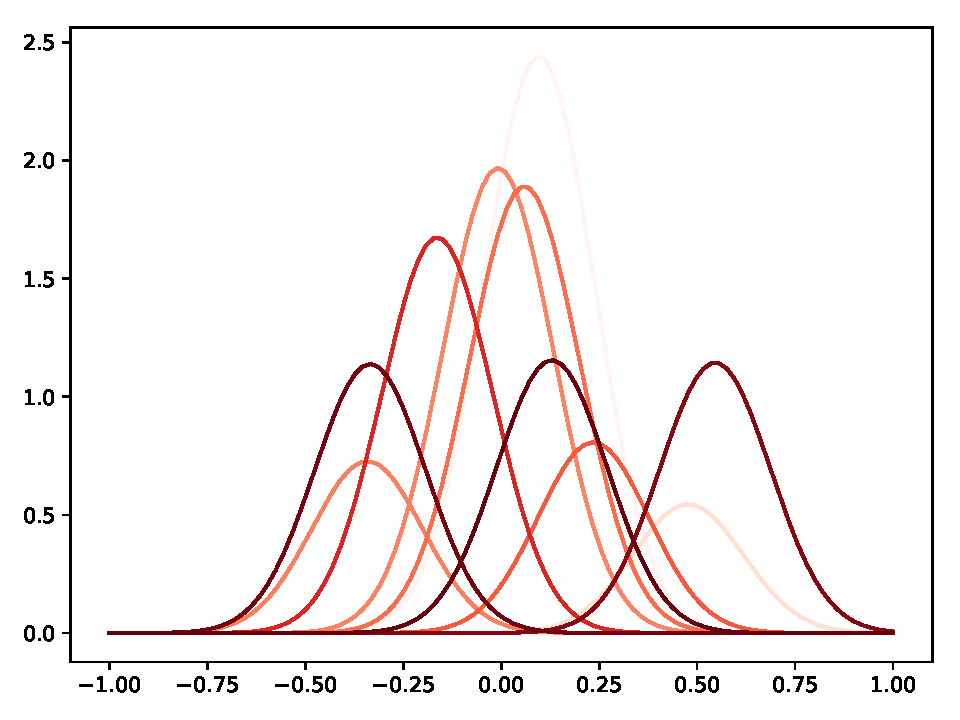
\includegraphics[width=7cm]{dataset-by-amplitude}} \quad
	\subfigure[SBFIG:RANK2]{Ranked by phase distance}{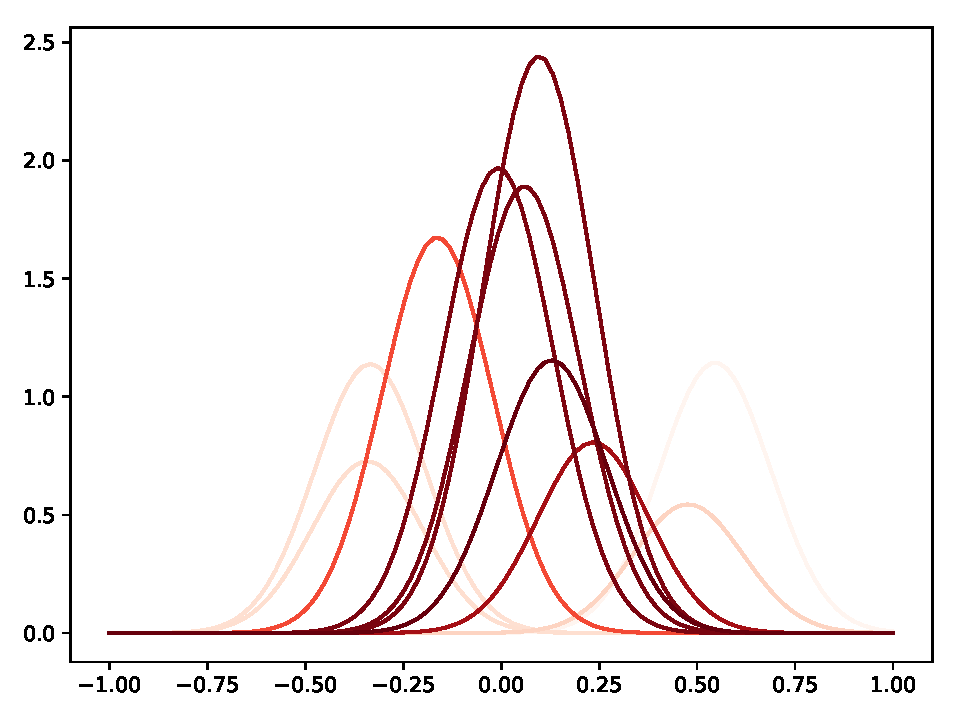
\includegraphics[width=7cm]{dataset-by-phase}}
\end{figure}

The Fréchet mean of these random points will be defined as the element $m \in X$
which globally minimizes the Fréchet Variance. If this global minimum does not
exist, we will call Karcher means to the points that locally minimizes the variance
$\Psi(p)$, i. e.,

\begin{equation}[]{Karcher means}
m=\underset{p \in M}{\arg \min } \sum_{i=1}^{N} d^{2}\left(p, x_{\dot{i}}\right)
\end{equation}

These Karcher means are adapted to the metrics used in the analysis. For this reason they can better capture the geometry of our problem
than usual mean, as it is shown in the Figure \ref{SBFIG:KARCHER2}, where it is
used a Karcher mean on $\mathscr{A}$.
%To calculate these means are used the algorithms explained in the appendix \ref{SEC:KARCHERF}.
The dataset shown in \ref{SBFIG:KARCHER1} contains Gaussian-like
samples, however the usual mean of Figure \ref{SBFIG:KARCHER2} is not able to reflect
this shape, unlike the Karcher mean in $\mathscr{A}$.



As an example of the behavior of these means with different metrics,
the centrality of an observation in a dataset  can be measured using its
distance to the Karcher mean. In the Figure \ref{FIG:KARCHER} it is used this idea to rank a dataset of
unimodal samples. Reddish colors indicate higher centrality of a sample, i.e.,
a smaller distance to the mean, and lighter colors indicates outlier samples.
In the Figure \ref{SBFIG:RANK1} it is used the amplitude distance, and their
corresponding Karcher mean. We can observe that the location of the mode in a
sample does not affect its centrality, in contrast to the phase distance,
as it is shown in the Figure \ref{SBFIG:RANK2}.
